\section{Спектральная структура и бифуркации}

В этом разделе исследуется эволюция спектра мультипликаторов Флоке вдоль семейства орбит. Показано, что топология спектра претерпевает качественные изменения, которые, однако, не всегда сопровождаются изменением устойчивости.

\subsection{Общая карта спектров и показателя Ляпунова}
В зависимости от расположения мультипликаторов на комплексной плоскости все орбиты в исследуемом семействе делятся на три класса: C, R и OTHER (см. раздел 2). 
На рисунке~\ref{fig:lambda_T_kind} показана зависимость показателя Ляпунова \(\lambda = \ln(\max |\mu|) / T\) от периода \(T\), раскрашенная по типу спектра. Видно, что орбиты типа C и R занимают непересекающиеся области, а тип OTHER (характерный для блока \textit{canonical} и начала \textit{near\_bif}) плавно переходит в них. Показатель \(\lambda\) монотонно убывает вдоль семейства от \(\approx 1.95\) (в начале блока \textit{canonical}) до \(\approx 0.3\) (в блоке \textit{arclength}).

\begin{figure}[H]
    \centering
    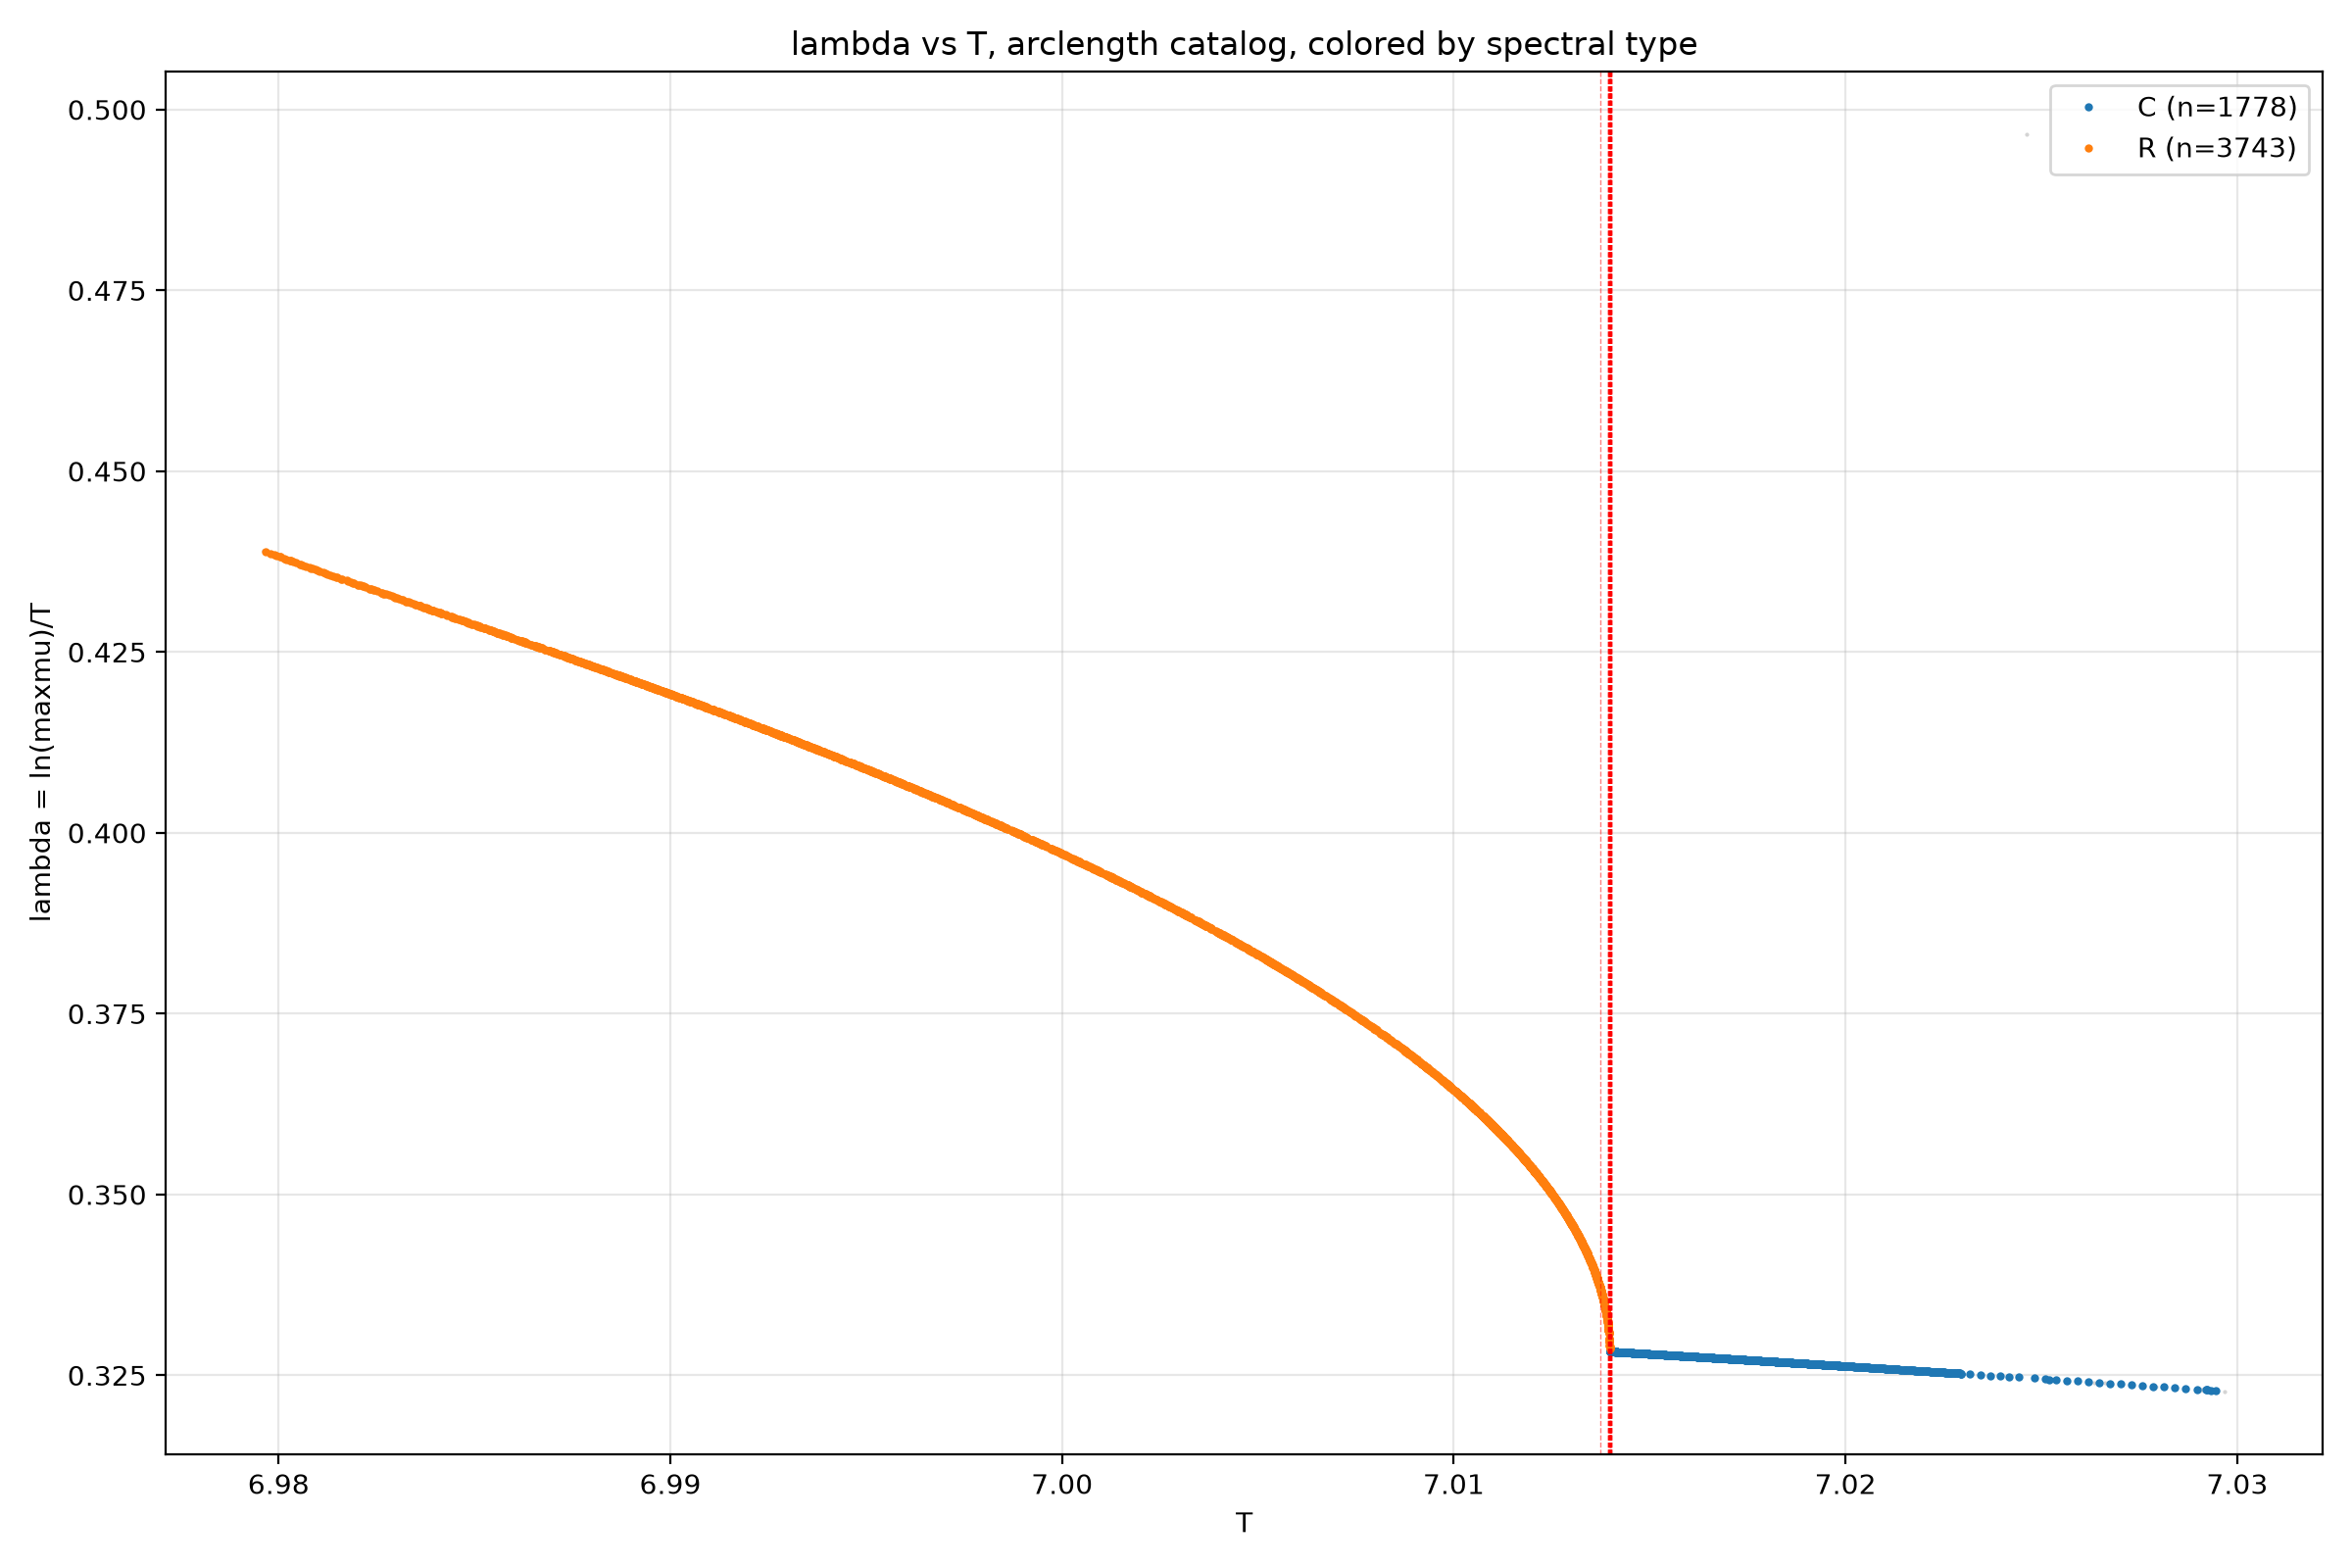
\includegraphics[width=0.85\textwidth]{30_lambda_T_kind.png}
    \caption{Зависимость показателя Ляпунова \(\lambda\) от периода \(T\). Цветом обозначен тип спектра (C, R, OTHER).}
    \label{fig:lambda_T_kind}
\end{figure}

\subsection{Единственное окно устойчивости в блоке unified}
В каталоге \texttt{catalog\_unified.tsv} было найдено единственное окно устойчивости, в котором все восемь мультипликаторов Флоке лежат на единичной окружности (т.е. \(\max |\mu| = 1\)). Это окно соответствует индексам \(gidx \in [15690, 15767]\) (периоды \(T \in [6.852, 6.989]\)).

Вход в это окно сопровождается переходом типа OTHER \(\to\) C. При \(gidx = 15690\) происходит следующее: вещественная пара мультипликаторов подходит к точке \(\mu = +1\), сливается с комплексной парой и обе уходят на единичную окружность. Этот процесс известен как \textbf{1:1 резонанс} или \textbf{столкновение Крейна} (Krein collision). 

Структура Жордана для мультипликатора \(\mu=1\) во всём семействе (кроме самой точки равновесия \(gidx=0\)) имеет вид \(J_2 + J_2\) (две жордановы клетки размера 2). Это стандартная структура для однопараметрического семейства в гамильтоновой системе, указывающая на отсутствие скрытых симметрий, порождающих дополнительную кратность. Точный переход OTHER \(\to\) C показан на рисунке~\ref{fig:other_c_transition}.

\begin{figure}[H]
    \centering
    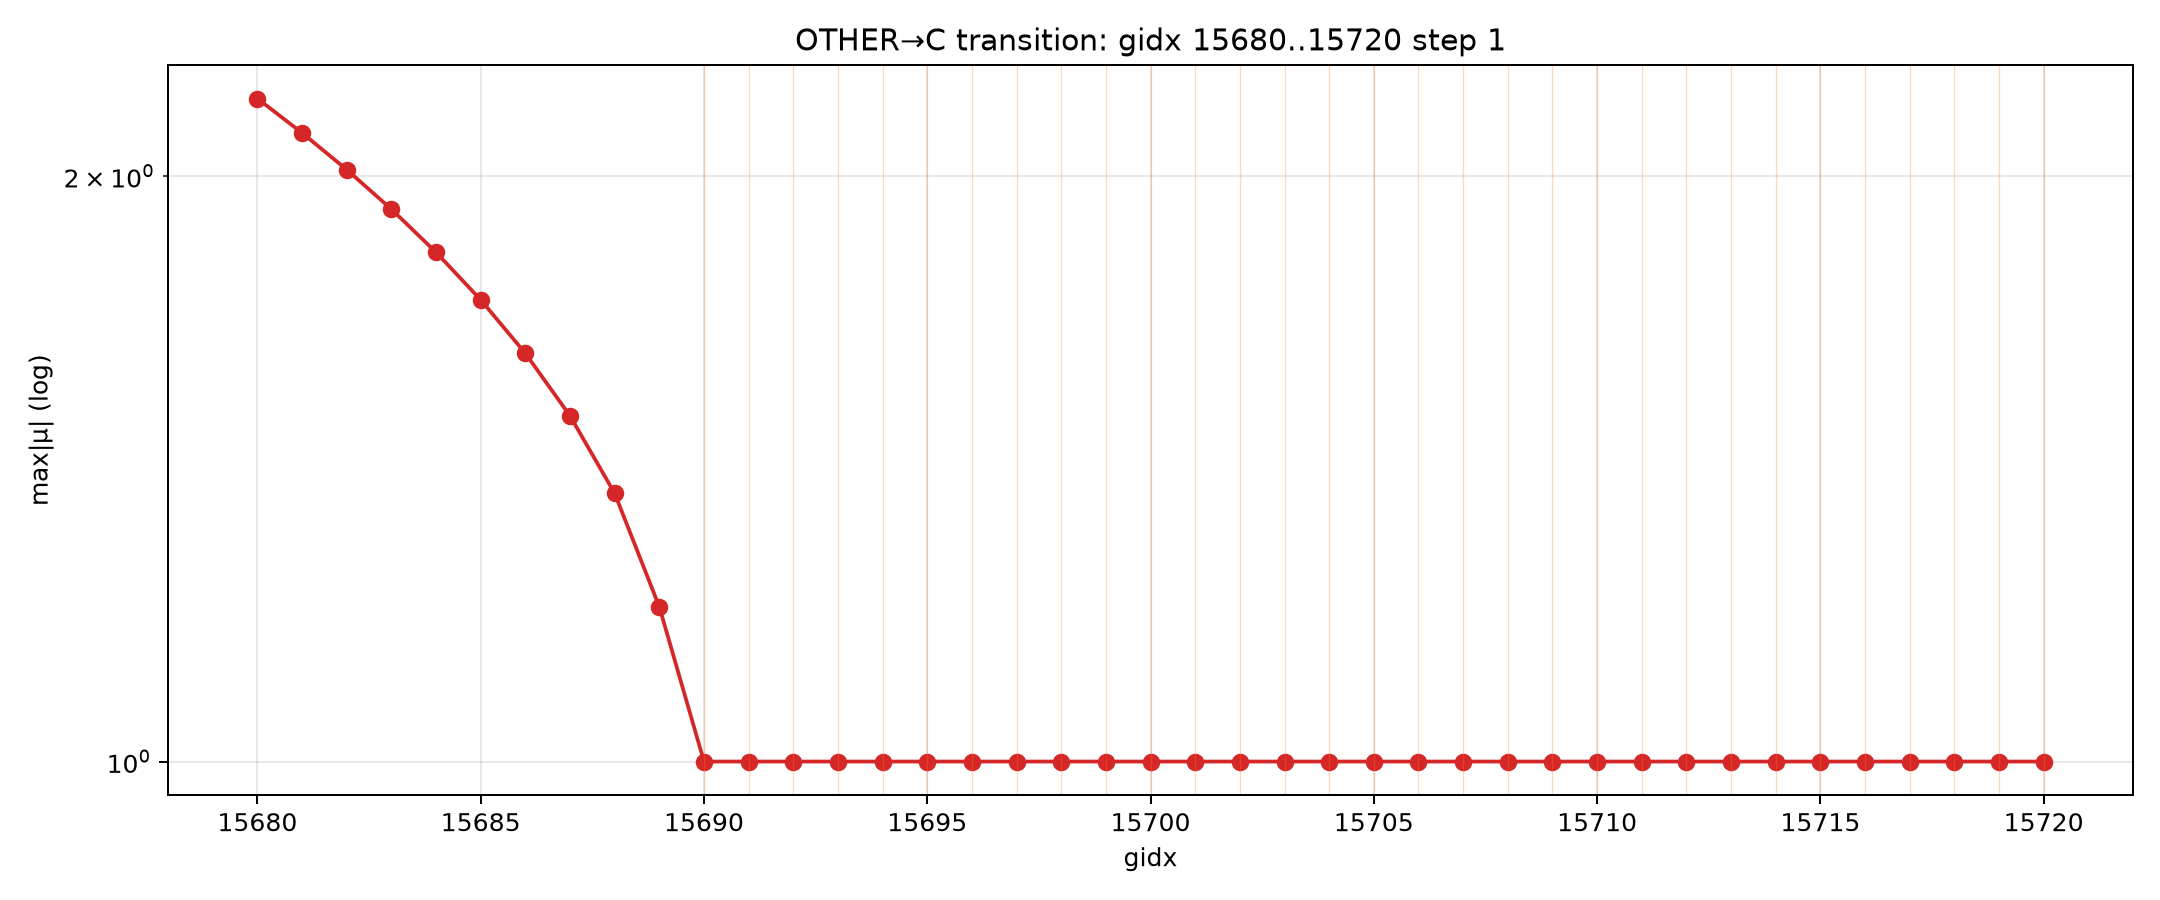
\includegraphics[width=0.85\textwidth]{88_other_c_transition.png}
    \caption{Точный переход OTHER \(\to\) C в блоке \textit{long} при \(gidx = 15690\) (1:1 резонанс) и последующее окно устойчивости.}
    \label{fig:other_c_transition}
\end{figure}

\subsection{Переходы C \(\leftrightarrow\) R в блоке arclength}
В блоке \textit{arclength} было зафиксировано 14 C-окон и 13 R-окон, которые строго чередуются. Всего найдено 27 переходов C \(\leftrightarrow\) R. 

Механизм всех этих переходов одинаков: пара комплексно-сопряжённых мультипликаторов с модулем \(\approx 0.100\) движется по комплексной плоскости, при подходе к вещественной оси их мнимая часть обращается в нуль, и они образуют вещественную пару \((\mu, 1/\mu)\). При этом \textbf{устойчивость орбиты не меняется}: показатель \(\lambda\) остаётся непрерывным, меняется лишь топология расположения мультипликаторов. В блоке \textit{long} (unified) переходов C \(\leftrightarrow\) R нет.

\subsection{Критический показатель \(\beta = 1/2\)}
Для количественного описания перехода C \(\leftrightarrow\) R рассмотрим поведение мнимой части мультипликатора вблизи точки бифуркации \(idx_c\). Было проверено 25 границ перехода. Для 17 из них линейная зависимость
\begin{equation}
    \text{Im}(\mu)^2 = a \cdot |idx - idx_c|
\end{equation}
выполняется с коэффициентом детерминации \(R^2 > 0.99\). Это подтверждает критический показатель \(\beta = 1/2\), характерный для слияния двух собственных значений на вещественной оси (седло-узловая бифуркация в терминах мультипликаторов). Результат линеаризованного коллапса показан на рисунке~\ref{fig:beta_collapse}.

\begin{figure}[H]
    \centering
    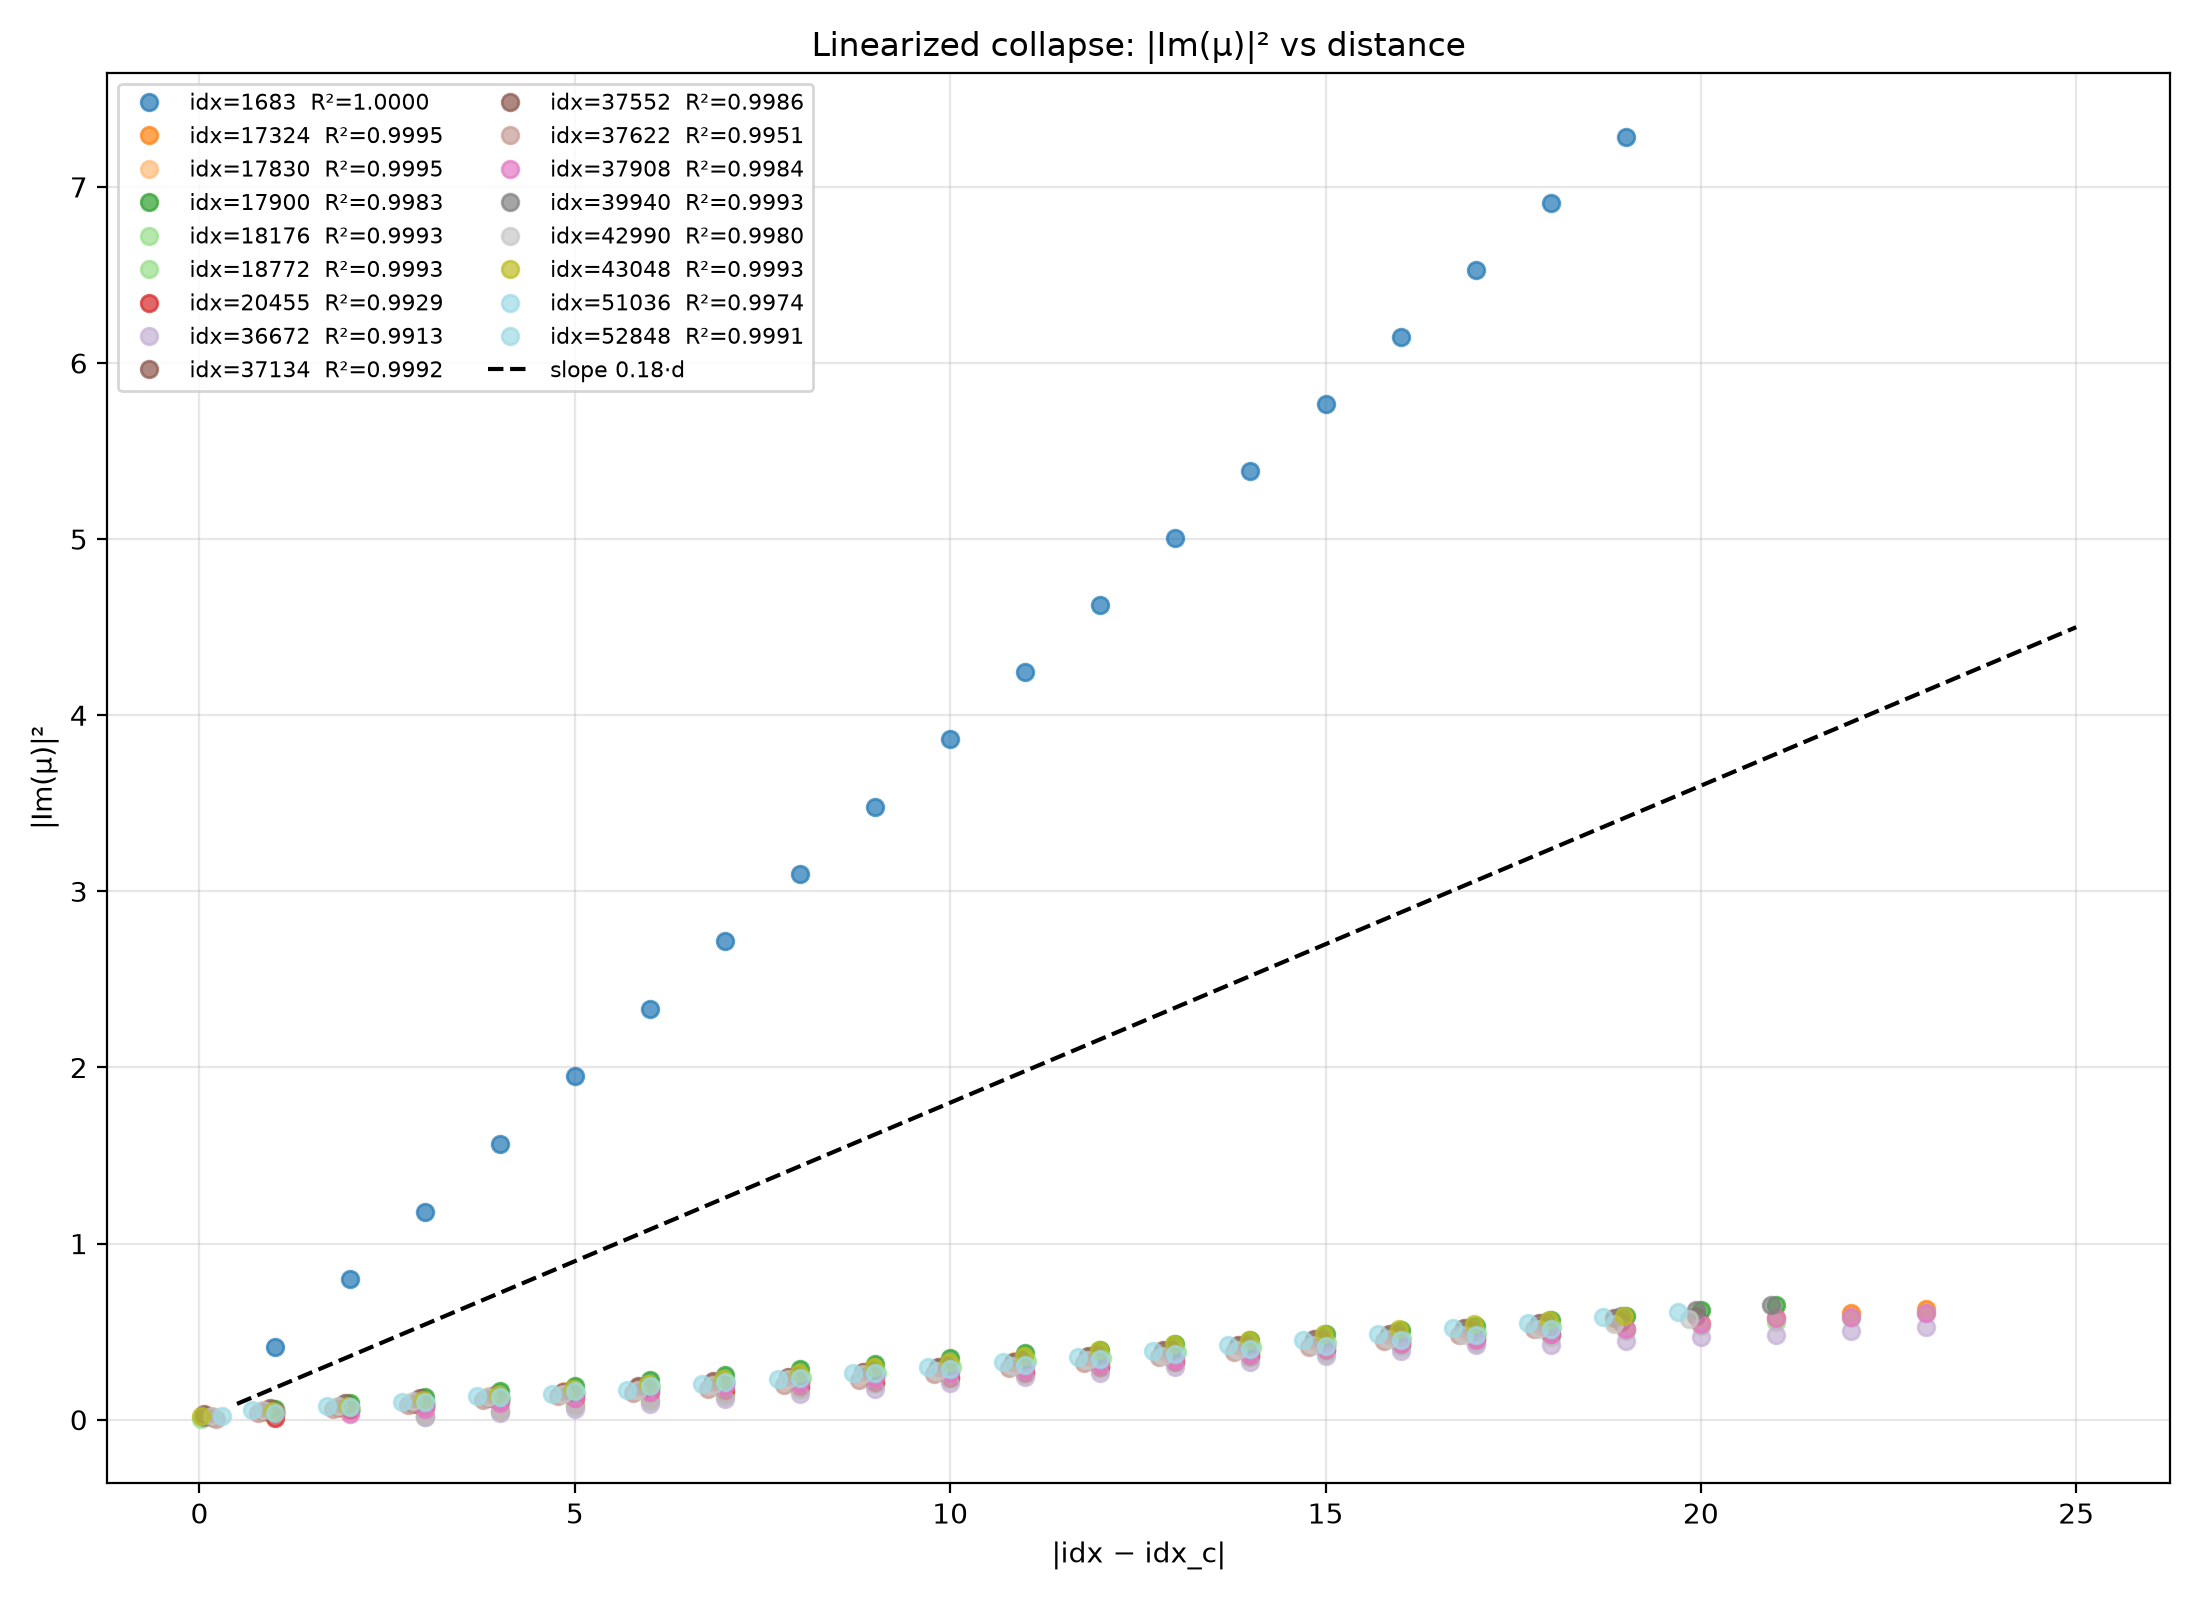
\includegraphics[width=0.8\textwidth]{39_linearized_collapse.png}
    \caption{Линеаризованный коллапс \(\text{Im}(\mu)^2\) от расстояния до точки перехода \(|idx - idx_c|\) для 17 границ C\(\leftrightarrow\)R. Наклон прямых соответствует \(\beta = 1/2\).}
    \label{fig:beta_collapse}
\end{figure}
